Flytt BNC-T leddet fra MAIN OUT til AUX OUT/TTL/CMOS.
Dette gir et firkantsignal (TTL-signal) som skifter mellom 0V og 5V.
Sett frekvensen til 1kHz.



\subsection{Oppg 4a}
Finn høyeste frekvens DTL-kretsen klarer å gjengi.
Det vil si frekvensen hvor ikke lenger utgangspulsene overstiger
halve inngangsspenningen.
\\\\
Vi justerte frekvensen opp til 150kHz hvor vi så at utgangspulsene var halveis
på inngangspulsen.
\begin{figure}[H]
  \caption{Høyeste gengivbare frekvens.}
  \centering
    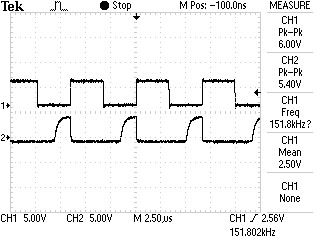
\includegraphics[width=\textwidth]{4a.jpg}
\end{figure}
Komponentene i kretsen bruker litt tid på å reagere.
Og på et tidspunkt vil inngangsfrekvensen være så hyppig at komponentene
ikke lenger rekker å reagere fort nok.



\subsection{Oppg 4b}
Vi stiller signalet til 100kHz og stiller inn cursoren.
Forsinkelsen før reaksjon er på 1,92us eller 1920ns.
\begin{figure}[H]
  \caption{Forsinkelse i kretsen.}
  \centering
    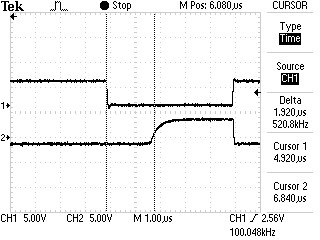
\includegraphics[width=\textwidth]{4b.jpg}
\end{figure}
Transistor opererer i metning og bruker tid på å gjenopprette
sperresjikte mellom base og collector.
\\\\
I motsatt retning retning er forsinkelsen \emph{mye} mindre.
Vi måler 28ns.
\begin{figure}[H]
  \caption{Forsinkelse i kretsen.}
  \centering
    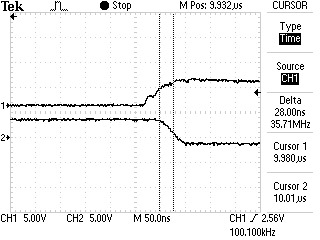
\includegraphics[width=\textwidth]{4bb.jpg}
\end{figure}
